%%%%%%%%%%%%%%%%%%%%%%% file template.tex %%%%%%%%%%%%%%%%%%%%%%%%%
%
% This is a general template file for the LaTeX package SVJour3
% for Springer journals.          Springer Heidelberg 2010/09/16
%
% Copy it to a new file with a new name and use it as the basis
% for your article. Delete % signs as needed.
%
% This template includes a few options for different layouts and
% content for various journals. Please consult a previous issue of
% your journal as needed.
%
%%%%%%%%%%%%%%%%%%%%%%%%%%%%%%%%%%%%%%%%%%%%%%%%%%%%%%%%%%%%%%%%%%%
%

\RequirePackage{fix-cm}
%
\documentclass{svjour3}                     % onecolumn (standard format)
%\documentclass[smallcondensed]{svjour3}     % onecolumn (ditto)
%\documentclass[smallextended]{svjour3}       % onecolumn (second format)
%\documentclass[twocolumn]{svjour3}          % twocolumn
%
\smartqed  % flush right qed marks, e.g. at end of proof
%
\usepackage{graphicx}
\usepackage{amsmath,amssymb}
%
% \usepackage{mathptmx}      % use Times fonts if available on your TeX system
%
\usepackage{cmap}
\usepackage[T2A]{fontenc}				% Поддержка русских букв
\usepackage[utf8]{inputenc}				% Кодировка utf8
\usepackage[english, russian]{babel}	% Языки: русский, английский

% Insert the name of "your journal" with
\journalname{Artificial Intelligence Review}

\begin{document}

\title{Multilayer cognitive architecture for AUV control\thanks{This work was supported by the Russian Scientific Foundation, project no. 14-11-00692.}
}

\author{Dmitry Makarov         \and
        Aleksandr Panov \and
        Konstantin Yakovlev
}

\institute{D. Makarov \and A. Panov \and K. Yakovlev\at
              Institute for Systems Analysis RAS, Moscow, Russia \\
              Tel.: +7-499-131273\\
              \email{makarov@isa.ru}           %  \\
}

\date{Received: date / Accepted: date}
% The correct dates will be entered by the editor

\maketitle

\begin{abstract}
Our abstract.
\keywords{First keyword \and Second keyword \and More}
\end{abstract}

\section{Introduction}
\label{intro}
Проектирование и разработка беспилотных транспортных средств различного типа и назначения – одна из наиболее динамично развивающихся областей в науке и технике в последнее время. К факторам, положительно влияющим на наблюдаемое ускорение прогресса в этой области, можно отнести: миниатюризацию датчиков, улучшение их характеристик, удешевление компонентной базы, повышение производительности бортовых вычислителей и др. Одна из тенденций последнего времени – появление унифицированных робототехнических платформ, оснащенных необходимым набором датчиков и исполнительных механизмов (актуаторов), а также программным обеспечением с открытыми интерфейсами (API), позволяющих исследователям сосредоточиться непосредственно на программной реализации системы управления (СУ) аппаратом. Если говорить о беспилотных летательных аппаратах (БЛА), то к таким платформам, пользующимся большой популярностью, можно отнести AR.Drone [1, 2], mikrokopter [3]. Характерно, что обе эти платформы представляют собой малые квадрокоптеры (вес – менее килограмма, размеры – не более 50 см. в диаметре), т.е. винтокрылые аппараты вертикального взлета и посадки с числом винтов 4-6 шт.

Стоит заметить, что в последнее время наблюдается смещение интересов роботехнического сообщества от колесных роботов к летательным аппаратам (ЛА), т.к. первые изучаются уже достаточно давно и считается, что задача создания беспилотного, полностью автономного колесного аппарата (например, на базе серийного автомобиля) принципиально решена, что подтверждается успешным завершениям ряда масштабных проектов в этой сфере (см. например результаты одного из последних соревнований беспилотных автомобилей DARPA Urban Challenge [4]). Задача же автоматизации управления объекта со сложной нелинейной динамикой в трехмерном пространстве на текущий момент не решена. И именно c решением этой задачи связывают существенный прогресс в области создания новых методов и алгоритмов распознавания образов, управления, планирования траектории, построения модели мира и др.

В данной работе под БЛА понимается в первую очередь малый квадрокоптер, такой как, например, уже упомянутый AR.Drone. При этом описываемые в статье принципы построения архитектуры СУ БЛА применимы и для других типов ЛА как то: БЛА классических вертолетных компоновок (с одним несущим и одним рулевым винтами, с двумя несущими соосными винтами), БЛА самолетного типа и др. 

\section{Recent works}
\label{sec:1}

Одним из наиболее распространенных подходов к построению архитектуры программной системы управления БЛА является подход, основанный на функциональный декомпозиции, когда СУ представляет собой совокупность взаимно-увязанных программных модулей, каждый из которых предназначен для решения определенного типа задач. Число таких модулей и принципы их связывания в единую структуру в общем случае не регламентированы. Заметим, однако, что в конце 90-х годов ХХ века принимались определенные попытки стандартизации в этой сфере. Так можно отметить стандарт JAUS [5], определяющий протоколы и форматы межмодульных взаимодействий. Предполагалось, что следование этому стандарту обеспечит возможность создания СУ путем включения модулей от различных разработчиков, а также «быстрой замены» модулей в случае необходимости.

При модульной декомпозиции, обычно выделяются следующие классы задач:
\begin{itemize}
	\item планирование – составление планов достижения целей и решения поставленных задач;
	\item взаимодействие – формирование групп БЛА и обеспечение взаимодействия между членами групп;
	\item управление в нештатных ситуациях – идентификация, анализ и ликвидация последствий возникающих незапланированных/нештатных ситуаций;
	\item оценка обстановки  – формирование модели мира;
	\item управление коммуникациями  – обеспечение взаимодействия с коммуникационными системами БЛА;
	\item управление БЛА – планирование траектории (с учетом рельефа, препятствий и динамики вертолета), управление системами и узлами вертолета, датчиками, оружием;
	\item управление ресурсами – управлением вычислительными ресурсами, распределение ресурсов между компонентами системы.
\end{itemize}

Пример СУ БЛА, состоящей из модулей, предназначенных для решения вышеприведенных классов задач, описан в [6].

В начале 2000х годов, в национальном институте стандартизации США (NIST) под руководством профессора Альбуса (Albus) функционировала группа, занимающаяся разработкой концептуальной модели архитектуры СУ для беспилотной техники, которая бы не опиралась на функционально-модульную декомпозицию. Такая концептуальная модель архитектура была создана и получила название 4D/RCS [7].

Основным структурным элементом 4D/RCS является узел, определяемый как совокупность четырех процессов системы управления:
\begin{itemize}
	\item обработка сенсорной информации;
	\item построение модели мира;
	\item оценивание свойств;
	\item выбор управляющих воздействий (генерация поведения).
\end{itemize}

Фактически процесс в модели 4D/RCS – есть архитектурный модуль, основное отличие которого от модулей, описываемых выше – неявная типизация. То есть отдельный модуль, например, планирования или составления расписаний не предусматривается моделью, однако функционал последних включается в модуль генерации поведения.

Стоит отметить, что модель 4D/RCS предполагает возможность создания иерархий узлов (т.е. создания многоуровневых архитектур управления). При этом состав компонент узлов 4D/RCS не меняется от уровня к уровню, но меняется семантика протекающих в узлах процессов – например, на более высоком уровне управления под генерацией поведения понимается планирование поведения (действий), а на более низком – планирование траектории (перемещений).

Заметим, что идея многоуровневых архитектур не нова в робототехнике, искусственном интеллекте (ИИ), теории управления и смежных дисциплинах. Однако обычно, когда речь идет о разделении на уровни, выделяют два из них – делиберативный и реактивный [8]. Программные модули реактивного уровня, реализуют непосредственно управление исполнительными механизмами беспилотного аппарата, а также «быструю» обработку информации для решения задач так или иначе связанных с поддержание заданных параметров (скорости, углового положения и т.д.). На делиберативном уровне выполняются задачи построения модели мира, оценки обстановки, планирования и т.д. Важным вопросом при таком подходе является принцип организации взаимодействия между двумя уровнями. Проработке этого вопроса посвящен ряд работ (например, обзор [9]), анализируя которые можно сделать вывод о том, что наиболее распространен следующий подход. Модули реактивного уровня являются полностью самодостаточными, то есть задачи, решаемые на этом уровне, имеют наивысший приоритет (например, задача поддержания заданной высоты и/или скорости). Результатом же функционирования модулей делиберативного уровня является формирование целей и задач на таком уровне абстракции, что они являются непосредственными входными данными для  реактивных модулей (например, «в течение 10 минут обеспечить зависание над заданной точкой»).

Можно утверждать, что к настоящему моменту применение одно- и двух-уровневых архитектур для построения систем управления беспилотной техникой нецелесообразно в силу следующих двух, взаимосвязанных факторов. Во-первых, возрастает объем данных, поступающих от датчиков объекта управления. Во-вторых, анализируя и обрабатывая определенным образом поступающие данные, становится возможным решение широкого спектра задач, объединение которых в рамках одного делиберативного уровня приводит к чрезмерному усложнению модульной архитектуры и дублированию модулей, концептуально предназначенных для решения единой задачи, но использующих для этого разные методы. В качестве примера можно привести задачу планирования, одновременно решаемую на делиберативном уровнях в разных контекстах (и разными методами) – контексте целей (планирование поведения) и контексте перемещений (планирование траектории). Соответственно целесообразным видится дальнейшее разбиение делиберативного уровня на подуровни: стратегический (ответственный за постановку и выбор целей, прогнозирование, и высокоуровневую обработку информации) и тактический (ответственный за распознавание образов, построение карты местности, планирование траектории и др.).

Итак, на основе проведенного анализа имеющихся подходов к построению архитектуры системы управления БЛА, можно сделать вывод о целесообразности применения трехуровневой архитектуры с выделением следующих уровней: стратегического, тактического и уровня управления. Основным отличием программных модулей расположенных на разных уровнях является степень обработки входящей информации и время отклика. Так на нижнем уровне (уровне управления) происходит оперативная обработка данных непосредственно поступающих от датчиков БЛА для решения задач выдерживания параметров управления. На среднем уровне (тактическом) происходит дальнейшая обработка информации и создание простейших информационных структур (графов, таблиц) для решения задач распознавания образов, построения модели местности, локализации, планирования траектории и др. На верхнем уровне (стратегическом) решаются задачи, требующие наибольшей степени обработки данных и создания сложных информационных структур (систем фреймов, неоднородных семантических сетей, систем правил и др.).


\section{General view of architecture}
\label{sec:2}
В ходе работ по проекту разработана концептуальная схема архитектуры системы управления, состоящая из трех уровней: стратегического, тактического и реактивного. Архитектура описывает (см. рис. \ref{fig:arch}) основные модули, выделенные в соответствии с функциональными возможностями каждого из уровней, а также взаимодействие между ними (вид и направление передаваемых данных). 

\begin{figure}
	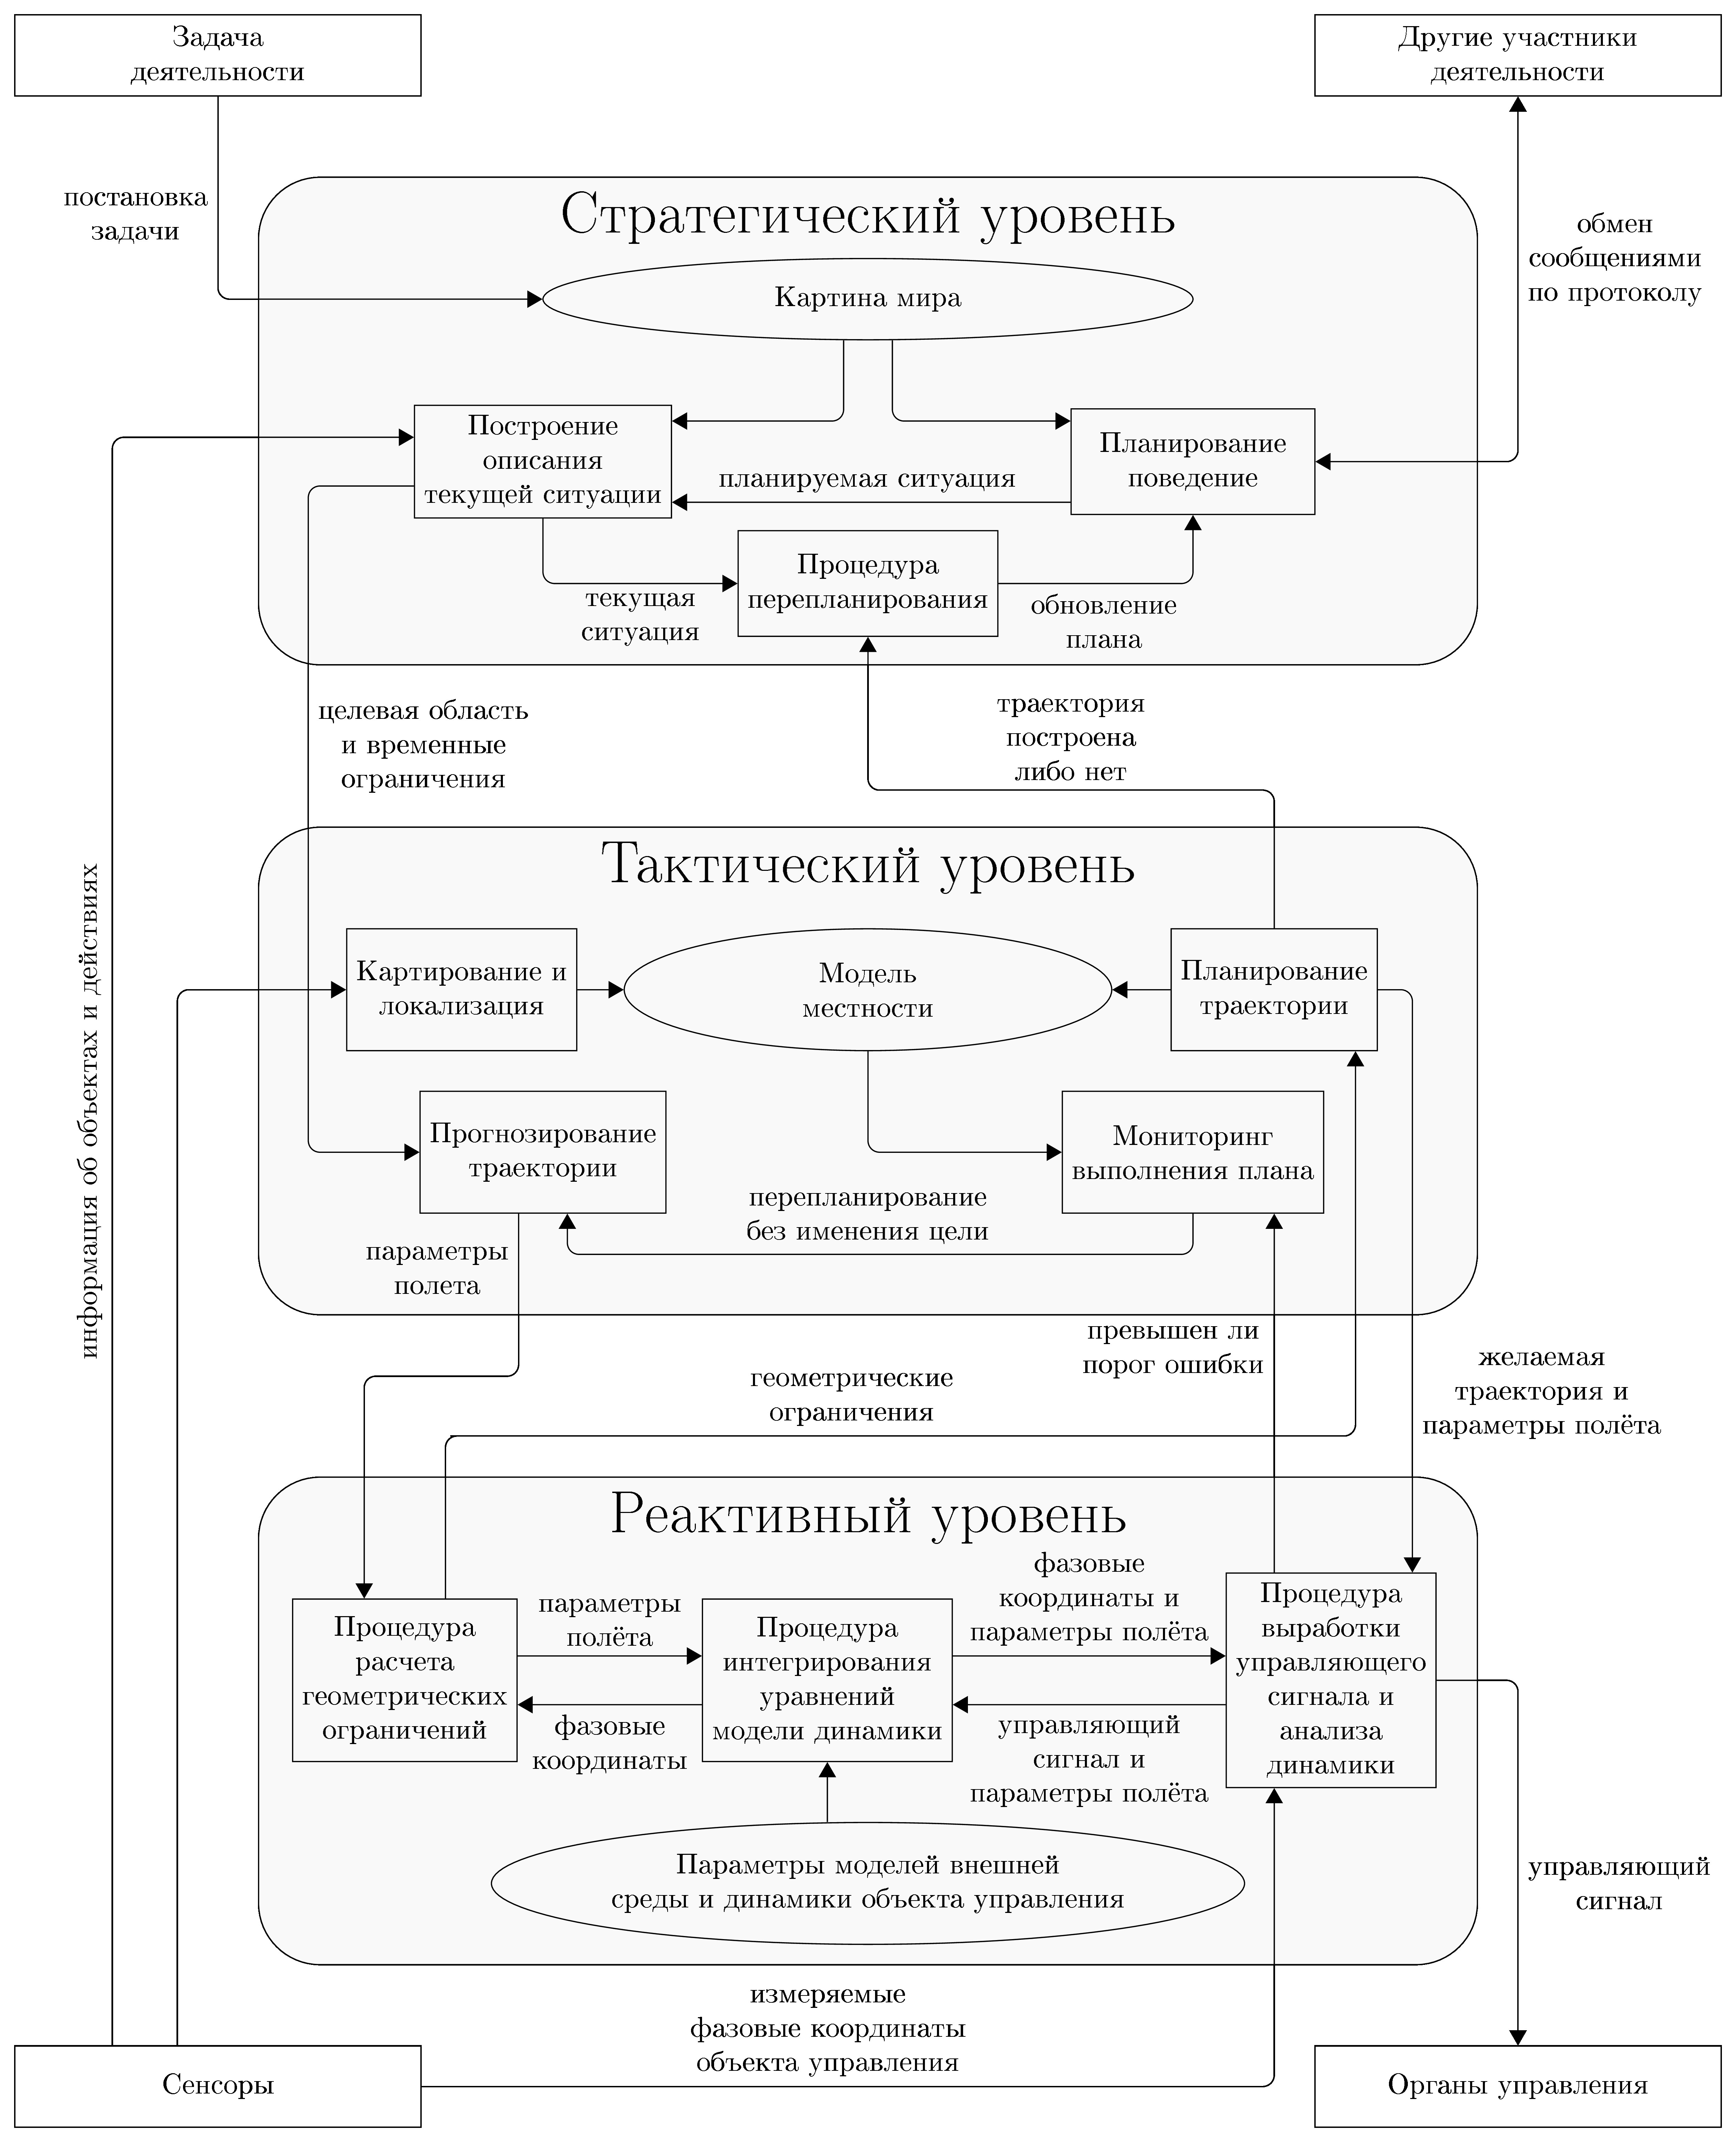
\includegraphics[width=\textwidth]{../../images/architecture-0}
	\caption{Schema of proposed congitive architecture.}
	\label{fig:arch}
\end{figure}

Основной задачей управление на стратегическом уровне является построение согласованного между членами коалиции плана поведения каждого участника совместной деятельности. Каждый участник обладает собственной картиной мира, которая специфична благодаря как характерным свойствам, ограничивающим множество доступных системе управления действий, так и компонентами элементов картины мира. Компоненты значения всех элементов картины мира для всех участников коалиции одинаковы по определению.

Построение плана поведения происходит за счет обмена сообщениями с другими участниками коалиции. На каждом этапе выполнения плана происходит обновление описания текущей ситуации, в том числе и с участием информации, поступающей от сенсоров. Из описания текущей ситуации выделяется пространственно-временная информация, которая формирует задание, поступающее на тактический уровень управления и содержащее пространственное описание целевой области и временные ограничения на её достижение.

Процедура перепланирования принимает результат о возможности или невозможности с заданными ограничениями выполнить задание по перемещению и при необходимости вносит согласованные с остальными участниками коалиции коррективы в общий план.

На тактическом уровне управления решаются задачи навигации объекта управления в пространстве, основными из которых являются: картирование (построение, обновление, уточнение модели (карты) местности), локализация (привязка объекта управления к имеющейся карте) и планирование траектории. Последняя задача разбивается на 3 фазы: прогнозирование, непосредственно построение плана и мониторинг. В модуль прогнозирования поступает информация со стратегического уровня управления о целевой области пространства и временных ограничениях на достижение этой области объектом управления, после чего осуществляется предварительный расчет необходимых параметров движения (например - скорости) для выполнения поставленного задания. Основное отличие методов прогнозирования траектории от методов собственно планирования заключается в том, что первые могут пренебрегать ограничениями на динамику движения объекта управления и другими ограничениями. За счет этого прогнозирование траектории осуществляется с минимальными затратами вычислительных ресурсов. Рассчитанные модулем прогнозирования параметры движения передаются на нижний (реактивный) уровень управления, на котором уже осуществляется учет ограничений на динамику движения объекта управления. В результате формируются геометрические ограничения на форму траектории, соблюдение которых гарантирует возможность следования по ней при фиксированных, рассчитанных ранее параметрах движения (скорости). Модуль планирования строит траекторию с учетом этих геометрических ограничений. Результатом его работы является построенная траектория (тогда на верхний уровень передается соответствующее сообщение), либо сигнал о том, что при заданных ограничениях задача планирования траектории невыполнима (за отведённое время). В последнем случае на стратегический уровень передается запрос на перепланирование, т.е. на выбор другой целевой области в пространстве и/или других временных ограничений. Таким образом, планирование траектории представляет собой итеративный процесс с обратными связями как от верхнего, так и от нижнего уровней управления, что является существенным отличием предлагаемой архитектуры от современных аналогов. Предполагается, что использование итеративной петли “прогнозирование - расчет геометрических ограничений - планирование траектории - планирование поведения” позволит существенно повысить качество решения задачи интеллектуального управления сложными техническими объектами, т.е. позволит решать такие задачи, которые не могут быть решены в рамках имеющихся подходов.
Основной задачей управление сложным техническим объектом на реактивном уровне является обеспечение заданных характеристик динамического объекта с помощью управляющего воздействия по принципу обратной связи. Для этого в процедуру выработки управляющего сигнала с тактического уровня поступают желаемая траектория и желаемые параметры движения (например, скорость). Уровень может работать в двух режимах: управления реальным объектом и численного моделирование процесса управления.

В первом случае информация о текущих характеристиках динамического объекта (фазовые координаты) поступает от сенсоров, а управление подается на органы управления. Во втором - информация о текущих характеристиках динамического объекта поступает от процедуры интегрирования уравнений модели динамики полета, в нее же передается и текущее управляющее воздействие.

На реактивном уровне также с помощью соответствующей процедуры решается задача определения геометрических ограничений на допустимую траекторию перемещения. Для чего в эту процедуру с тактического уровня от модуля прогнозирования поступают желаемые параметры движения, которые передаются далее в процедуру интегрирования уравнений модели. На основании анализа полученных фазовых координат определяются геометрические ограничения, которые передаются обратно на тактический уровень в модуль планирования траектории.

Кроме того, на тактическом уровне происходит анализ ошибки управления, т.е.  на сколько фазовые координаты объекта (реально измеренные или полученные в ходе численного моделирования) отличаются от заданных. Ошибка сравнивается с допустимым порогом, результат сравнения передается на тактический уровень в модуль мониторинга выполнения плана.


\section{Details of organization of strategic level}
\label{sec:3}
\subsection{Knowledge representation}
В качестве базовых психологических теорий, в которых дается не только качественное описание свойств когнитивных функций, но и приводятся структурные описания лежащих в их основе психических образований, были использованы культурно-исторический подход Выготского-Лурии [1,2], теория деятельности Леонтьева [3] и модель психики Артемьевой [4]. Согласно приведенным теориям высшие сознательные когнитивные функции осуществляются в рамках так называемой мотивированной предметной деятельности, когда объекты и процессы внешней  среды опосредованы для субъекта специальными образованиями, называемыми знаками. Процесс задействования знака в той или иной когнитивной функции имеет три образующих: образ, значение и личностный смысл. Образная составляющая отвечает за функции воспроизведения и разлиичения опосредуемого предмета или процесса в ходе деятельности. Составляющая значения представляет собой место данного знака в той или иной надпсихологической знаковой системе, которая отражает в функциональном смысле наработанные общей исторической практикой коллектива-владельца данной знаковой системы способы использования опосредуемого предмета или процесса. Наконец, составляющая личностного смысла несет в себе собственный опыт действования субъекта с денотатом знака, который выражается в том числе и в интегральной оценке роли этого денотата в его текущей деятельности: способствует ли данные процесс или предмет удовлетворению текущего мотива.

Трехкомпонентная структура элемента индивидуального знания, которая как было сказано выше, в психологии называется знаком, подтверждается и теми работами нейрофизиологов, в которых предпринимается попытка построить общую теорию работы мозга человека. Так в теории повторного входа Эделмена [5] и Иваницкого [6] утверждается, что образование осознанного ощущения или фиксация входного потока информации происходит только в том случае, когда активированное сенсорным входом возбуждение через ассоциативные зоны коры от гиппокампа, а затем от гипоталамуса накладывается на сенсорный след в проекционной коре. Такой «круг ощущений», проходящий за характерное время в 150-300 мс, последовательно активирует три компоненты индивидуального знания: образную (проекционная и сенсорная зоны коры), компоненту значения (гиппокамп) и личностного смысла (гипоталамус).
Кроме того, по современным нейрофизиологическим представлениям строение коры головного мозга практически однородно во всем своем объеме (наличие колонок неокортекса). При этом множество связей между достаточно малыми зонами коры (так называемый коннектом) явно указывают на иерархичность ее строения и на присутствие как восходящих, так и обратных, нисходящих связей. Отсюда следует, что компоненты элемента индивидуального знания должны обладать иерархическим однородным строением с восходящими потоками информации и нисходящей обратной связью. Кроме того, образная компонента должна иметь такую функцию распознавания, которая кроме категоризации статических объектов и динамических процессов использует обратную связь для предсказания сигнала в следующий момент времени.

В качестве математической модели базовой составляющей всех компонент элемента индивидуального знания был предложен следующий бесконечный автомат Миля с переменной структурой и конечной памятью (распознающий автомат или $R$ -автомат):

\[
	R_{i}^{j}=X_{i}^{j}\times \hat{X}_{i}^{j+1}{{,2}^{\mathcal{Z}_{i}^{j}}},X_{i}^{*j}\times \hat{X}_{i}^{j},\varphi _{i}^{j},\vec{\eta }_{i}^{j},
\]
где $i$ – сквозной индекс автомата в иерархии, $j$ – уровень иерархии, $X_{i}^{j}$ – множество входных сигналов, $X_{i}^{*j}$ – множество выходных сигналов, $\hat{X}_{i}^{j+1}$ – множество управляющих сигналов с верхнего уровня иерархии, $\hat{X}_{i}^{j}$ – множество управляющих сигналов на нижний уровень иерархии, ${{2}^{\mathcal{Z}_{i}^{j}}}$ – множество состояний (множество подмножеств множества матриц предсказания (см. далее)), $\varphi _{i}^{j}:X_{i}^{j}\times \hat{X}_{i}^{j+1}\to {{2}^{\mathcal{Z}_{i}^{j}}}$ – функция переходов, $\vec{\eta }_{i}^{j}:{{2}^{\mathcal{Z}_{i}^{j}}}\to X_{i}^{*j}\times \hat{X}_{i}^{j}$ – вектор-функция выходов. Входные, выходные и управляющие сигналы представляют собой вектора действительных чисел, каждый компонент которых является весом распознаваемого или входного признака.

В качестве функции распознавания $k$-ого выходного признака ${{\hat{f}}_{k}}$ в $R$ -автомате удобно использовать набор булевых матриц предсказания ${{Z}_{k}}=\left\{ Z_{1}^{k},Z_{2}^{k},\ldots ,Z_{m}^{k} \right\}$, в которых каждый столбец $\bar{z}_{u}^{r}$ является вектором предсказания входных признаков в момент времени ${{\tau }_{s}}+u$, где ${{\tau }_{s}}$ – начало вычислительного цикла (момент действия управляющего сигнала $\hat{x}_{i}^{j+1}$). Сама матрица $Z_{r}^{k}$ задаёт последовательность битовых векторов, наличие бита в котором свидетельствует о присутствии распознаваемого функцией ${{\hat{f}}_{k}}$ признака. Алгоритм ${{\mathfrak{A}}_{th}}$ вычисления функции переходов $\varphi _{i}^{j}$ и выходной функции $\vec{\eta }_{i}^{j}$ по начальному моменту времени ${{\tau }_{s}}$, управляющему воздействию $\hat{x}_{i}^{j+1}({{\tau }_{s}})$ и входному воздействию $\omega _{i}^{j}$ представлен на рис 1.

Введение такого автомата и некоторых соотношений на множестве $R$ -автоматов позволяет определить все компоненты знака. Так, образом знака $s$, соответствующего признаку ${{f}_{1}}$, будет называться такое подмножество $p(s)$ признаков, что $\forall {{f}_{i}}\in p\left( s \right)~{{f}_{i}}\sqsubset {{f}_{1}}$. Здесь отношение $\sqsubset $ является отношением измеримости одного признака с помощью другого. Введение выделенных признаков–маркеров эффекта ${{f}_{e}}$ и условия ${{f}_{c}}$ ведет к следующему определению значения: если ${{f}_{1}}$– признак, соответствующий знаку $s$, ${{f}_{2}}$- процедурный признак, измеряющийся с помощью признаков–маркеров условия и эффекта, ${{f}_{1}}{{\sqsubset }^{c}}{{f}_{2}}$, то будем называть ${{f}_{2}}$ элементом значения признака ${{f}_{1}}$. Отношение ${{\sqsubset }^{c}}$ показывает, что признак ${{f}_{2}}$ сопутствует признаку-маркеру условия в матрице предсказания признака ${{f}_{1}}$. Наконец, введение выделенного подмножества личностных признаков ${{F}_{I}}$ приводит к определению личностного смысла: если ${{f}_{1}}$ – признак, соответствующий знаку $s$, ${{f}_{2}}$ - процедурный признак, ${{f}_{1}}{{\sqsubset }^{c}}{{f}_{2}}$, $\exists {{f}_{I}}\in {{F}_{I}}~{{f}_{I}}{{\sqsubset }^{c}}{{f}_{2}}$, то будем называть ${{f}_{2}}$ элементом личностного смысла признака ${{f}_{1}}$.


\subsection{Self-organized processes}
Между компонентами знака в процессе деятельности субъекта возникают определенные отношения, что, в свою очередь, приводит к формированию картины мира субъекта. В качестве модели картины мира субъекта деятельности были выбраны три типа семантических сетей: сеть на образах знаков, сеть на значениях и сеть на личностных смыслах. Процессы самоорганизации на этих сетях [7] включают в себя помимо пополнения семейств отношений также и образование новых узлов сети, что соответствует образованию нового элемента индивидуального знания. 

Процесс формирования нового знака включает в себя определение связей между компонентами знака, а затем именование получающейся структуры. До получения имени такая временная структура называется протознаком, а её компоненты: перцептом, который после завершения процесса формирования знака становится образом, функциональным значением, который становится значением, и биологическим смыслом, становящимся личностным смыслом. Общая схема образования нового знака выглядит следующим образом:
\begin{enumerate}
	\item Формирование перцепта.
	\item Порождение на основе прошлого опыта или на основе прецедентов - множества пар вида «перцепт - функциональное значение» - функционального значения объекта.
	\item Получение субъектом из культурной среды, аккумулированной в системе естественного языка, пары «имя знака – значение» и оценка специальным механизмом степени близости функционального значения, построенного на стадии 1 к значению, полученному из культурной среды; в случае недостаточной близости - переход к п. 1 и продолжение формирования перцепта.
	\item Связывание имени из пары «имя знака - значение» с перцептом, построенным после завершения выполнения п. 1–3; с этого момента перцепт превращается в образ.
	\item Формирование личностных смыслов знака на основе прецедентов действий с предметом.
	\item Связывание имени из пары «имя знака – значение» со сформированным личностным смыслом. С этого момента функциональное значение превращается в значение, а биологический смысл - в личностный смысл.
	\item Продолжение отображения «биологический смысл – перцепт» включением в область определения отображения личностного смысла, полученного в предыдущем пункте, а в область значений – образа из п. 4.
\end{enumerate}

Рассмотрение процедурных признаков в виде правил с определенными множествами добавляемых и удаляемых признаков позволяет сформировать алгоритм основного итерационного процесса (пп. 1-3 из вышеприведенной схемы) образования знака с помощью $R$ -автоматов (см. рис. 2). Для определения конфликтности и применимости правил на множестве процедурных признаков введены специальные операции приведения: сохраняющего приведения  столбца $\bar{z}$ к множеству признаков ($\bar{z}\to F$) и сужающего приведения двух столбцов (${{\bar{z}}_{1}}\Rightarrow {{\bar{z}}_{2}}$).


\section{Details of organization of tactic level}
\label{sec:4}

\section{Details of organization of reactive level}
\label{sec:5}

\section{Conclusion}
В последнее время наблюдается повышенный интерес к автономным летательным аппаратам вертолетного типа. Исследователями было предложено множество архитектур систем управления такими аппаратами. Большая сложность реализации автономных вертолетов приводит к тому, что двухкомпонентная архитектура систем управления, состоящая из делиберативного и реактивного уровней, становится неэффективной и появляется необходимость явного выделения иерархичной трехуровневой архитектуры, содержащей стратегический, тактический уровни и уровень управления. 

На стратегическом уровне осуществляется высокоуровневое планирование, в ходе которого стоится последовательность действий, решающих поставленную перед автономным летательным аппаратом задачу. Этот уровень является наименее проработанным, и существующие подходы обладают существенными недостатками. Преодоление основной трудности – проблемы автономного целеполагания – может быть достигнуто с помощью создания такого представление знаний, в котором описание действий с понятием, связи этого понятия с другими понятиями и процедуры выделения этого понятия из сообщений с нижележащего уровня управления представляли собой одну единицу знаний.

На тактическом уровне решаются задачи навигации БЛА и ключевой является задача построения траектории. Основная трудность, возникающая при решении последней, – громоздкость модели, описывающей трехмерную окружающую среду. Целесообразным способом преодоления указанной трудности является использование эвристических и декомпозиционных алгоритмов планирования.

На уровне управления основной задачей является построение регуляторов и наиболее перспективно развитие методов синтеза нелинейных робастных регуляторов с гладким управлением, обладающих строгим математическим обоснованием. Для улучшения работы полученных регуляторов возможно их совместное применение с механизмами адаптации (асимптотические наблюдатели, методы ИИ и др.), не нарушающих найденные условия устойчивости замкнутого контура. 

Разработанная архитектура позволяет решать большой спектр задач управления коалициями сложных технических объектов в динамической среде и будет использована для создания экспериментального образца программного обеспечения многоуровневой системы управления на следующих этапах работ по проекту.

% BibTeX users please use one of
\bibliographystyle{spbasic}      % basic style, author-year citations
%\bibliographystyle{spmpsci}      % mathematics and physical sciences
%\bibliographystyle{spphys}       % APS-like style for physics
\bibliography{3control}   % name your BibTeX data base

\end{document}


